\chapter{Results}

\section{Surviving Gadgets}

\begin{figure}[htp]
	\centering
	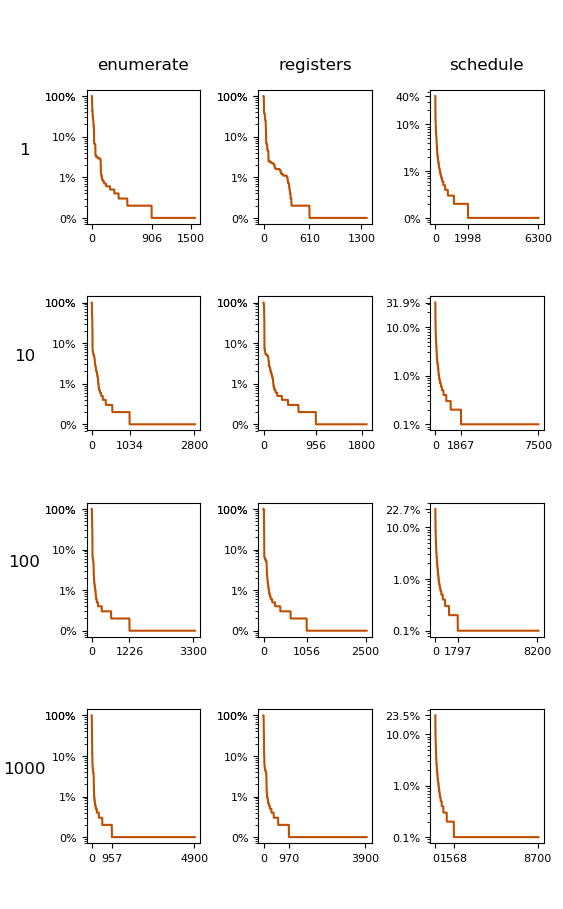
\includegraphics[width=\textwidth,height=\textheight]{results/figures/gadgets}
	\caption{The ratio of occurence for each gadget broken down by strategy and sampling rate.
	Each bar shows the occurence ratio for one particular gadget.}
	\label{fig:gadgets}
\end{figure}

Figure \ref{fig:gadgets} shows the occurence ratio of each gadget for the different
strategies and sampling rates. There were around 21000 gadgets in total for every program
across all versions. The x-axis shows a gadget id and there is no definitive correlation
between the gadgets across strategies and sampling rates. I.e gadget 0 for the enumerate
strategy at sampling rate 1 is not necessarily the same gadget 0 as the registers strategy
at sampling rate 10.

As seen in figure \ref{fig:gadgets}, neither the enumeration nor the registers strategy
were particularly effective at breaking gadgets for any sampling rate. There is a slight
improvement for higher sampling rates but it is not particularly impressive even at
sampling rate 1000. There are still many gadgets that appear in all programs.

Curiously, there seems to be little difference between sampling rate 10 and 100 for both
enumerate and registers. Sampling rate of 100 appears to be even worse at breaking gadgets
than sampling rate 10.

The schedule strategy seems to have performed very well. Not a single gadget was present
in even 50\% of all versions for any sampling rate. The strategy is even more effective at
higher sampling rates, which is in accordance with the expected behaviour described in
section \ref{sec:sampling_rate}.

\section{Cost}

The estimated cost of each program is shown in Figure \ref{fig:cost}. The dotted red line
shows the cost of the LLVM solution when calculated in the same manner.

\begin{figure}[h]
	\centering
	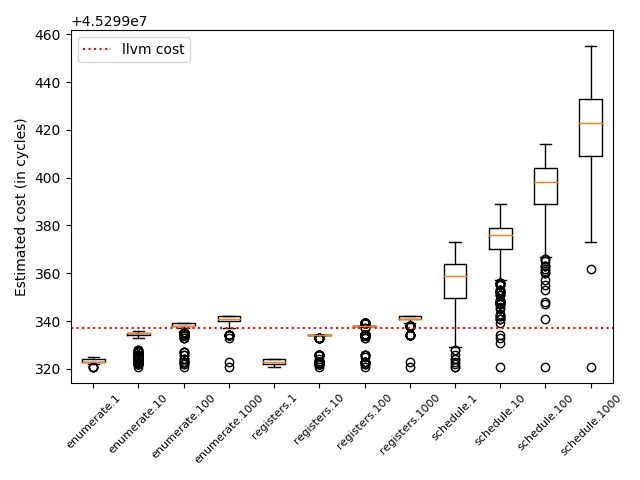
\includegraphics[width=\textwidth,height=0.5\textheight]{results/figures/cost}
	\caption{The cost distributions for every strategy and sampling rate. The cost of the LLVM solution is included for reference.}
	\label{fig:cost}
\end{figure}

All strategies perform better for lower sampling rates. As described in section
\ref{sec:performance} this is expected. Enumerate and registers perform equally well and
for sampling sizes of 1 and 10 they have a lower cost than the LLVM solution. The schedule
strategy seems to incur a significant overhead compared to the LLVM solution for all
sampling rates.

Interesting to note is that all strategies and sampling rates have found a solution with
an equally low cost. This is presumably the very first solution found; When no strategy
related constraints have been posted yet.


\section{Discussion}

What is interesting is that the registers strategy actually seem to perform \textit{worse}
than the enumerate strategy for the 10 and 100 sampling rates. This is surprising
because the versions of the registers strategy is theoretically a subset of versions of
the enumerate strategy.

% Remember to mention the hypothesis!!!

\section{Conclusion}

% Calculate the performance impact for carefully. Perhaps percentages in it's own plot?
To summarize the results and discussion it seems fair to draw the conclusion that enumerate
and registers, while incuring low overhead breaks very few gadgets and are thus not very
useful. The schedule strategy, however, performs very well when breaking gadgets but less
so regarding the cost. The cost of the schedule strategy varies greatly between sampling
rates, and for the lowest rate there is about 5\% performance impact for the mean.
